\chapter{Research methods}
\label{researchmethods}

 \lhead{\emph{Research methods}} % Chapter title for thesis template 

\section{Study design}
\label{studydesign}

This pilot study is a randomised crossover trial, utilising a bespoke, \href{http://respect.ambulanceresearch.co.uk}{web-based assessment tool}\footnote{\href{http://respect.ambulanceresearch.co.uk}{http:/\slash respect.ambulanceresearch.co.uk}} to enrol participants, randomise them appropriately, and track their progress through the study. The pilot has been designed to mirror the main study, enabling the testing of the assessment tool, data collection and analysis methods, and the statistical methods required for hypothesis testing.

\section{12-lead electrocardiograms}
\label{leadelectrocardiograms}

A key component of the assessment tool is a database of 48 12-lead ECGs showing a STEMI or STEMI-mimic waveform morphology. These are classified into four categories, based on the computer interpretation message on the ECG: true positive, true negative, false positive and false negative, when compared to the reference standard for ECGs in this study. Note that there are 12 ECGs for each classification.

\subsection{Reference standard}
\label{referencestandard}

In order to qualify for inclusion in the study, the ECGs had to meet the following reference standard set for the study:

\begin{itemize}
\item The ECG had to be a 12-lead ECG recorded in the out-of-hospital environment

\item The ECG had to display a wave morphology consistent with either a STEMI or STEMI-mimic, and a computer diagnostic message printed on the ECG.

\item The diagnosis of the ECG (i.e. STEMI or not-STEMI) had to be determined by the independent assessment and agreement of two senior doctors with specialist knowledge of ECGs. Any disagreements on diagnosis were resolved by discussion between the doctors. An option for subsequent review by an independent third party, was provided, but not required.

\end{itemize}

Information relating to the 48 ECGs that met the reference standard and were included in the pilot study, can be found in \autoref{appendixa}. 

\section{Participants}
\label{participants}

Participants for the pilot study were Health and Care Professions Council (HCPC) registered paramedics working in the United Kingdom, but not employed with Yorkshire Ambulance Service NHS Trust at the time of the study. The main study, planned to commence once the pilot data has been completed, will consist of Yorkshire Ambulance Service paramedics only. Approval has already been granted by the Service research and development department for the main study (\autoref{appendixc}). 

\section{Recruitment}
\label{recruitment}

A number of strategies were employed to recruit the target number of paramedics into the study. Firstly, the study was advertised on the \href{https://www.collegeofparamedics.co.uk/}{College of Paramedics website}\footnote{\href{https://www.collegeofparamedics.co.uk/}{https:/\slash www.collegeofparamedics.co.uk\slash }} (with the support of the College Research and Development Advisory Committee). In addition, paramedics were notified about the study via the \href{http://www.ukambulanceforum.com}{UK Ambulance Forum}\footnote{\href{http://www.ukambulanceforum.com}{http:/\slash www.ukambulanceforum.com}}, an online \href{http://www.resuscitate.me.uk}{continuing professional development portfolio builder}\footnote{\href{http://www.resuscitate.me.uk}{http:/\slash www.resuscitate.me.uk}} for ambulance staff, social media outlets such as \href{http://www.twitter.com}{Twitter}\footnote{\href{http://www.twitter.com}{http:/\slash www.twitter.com}}, email and word of mouth. 

\section{Ethical concerns}
\label{ethicalconcerns}

The confidentiality of the participants was maintained primarily through anonymity. The only potential source of personally identifiable data, the participant's email address, was encrypted on the pilot study database using a Rijndael 256-bit cypher and was not known to the researcher. In addition, there was no personal contact between participants and the researcher during the pilot study, since the website handled all communication with the participant, such as sending out reminder emails, for example. Access to the study database was limited to the chief investigator only. Once the study was completed, participants' email addresses and data were removed within one calendar month, unless express consent had been obtained from a participant to be contacted about involvement in a subsequent study.

The HCPC standards of conduct, performance and ethics, states that paramedic (and other) registrants must act in the best interests of service users, which includes reporting on the conduct, performance and health of colleagues if there is a cause for concern~\citep{health_and_care_professions_council_standards_2008}. This raised a potential ethical issue within the RESPECT pilot study, since paramedic participants' ability to interpret ECGs was tested, and since the chief investigator is a registrant of the HCPC, a dilemma about whether to report poorly performing participants arose. In actuality, since participants' identities were anonymised, and no overall score for an individual participant was calculated, it was not possible identify poorly performing participants individually.

Since the study was not conducted on NHS patients, there was no need for NHS research ethics committee (REC) approval as this is not required for research conducted on NHS staff~\citep{nhs_research_ethics_service_does_2012}. However, the study was approved by the University of Sheffield ethics committee (\autoref{appendixd}), and the University acted as the study's research governance sponsor (\autoref{appendixe}). In addition, a risk assessment was conducted, in keeping with University policy (\autoref{appendixf}). 

\section{Informed consent}
\label{informedconsent}

Participants in the RESPECT study consented online. Although, arguably, this raised an issue of ensuring that the participants were fully informed, comprehensive participant information was provided on the website (\autoref{appendixg}). Obtaining consent in this way, meant that no pressure to enrol in the study was exerted on the participant, which can occur in face-to-face consenting methods~\citep{fielding_handbook_2008}. Participants who submitted the consent form webpage (\autoref{consentform}), were considered to have provided informed consent. Additional consent was also obtained for the use of anonymised data from the study to be used in subsequent research, and for participants to be contacted for potential enrolment into a subsequent, qualitative study. These were both optional and not required to participate in the pilot.

\begin{figure}[htbp]
\centering
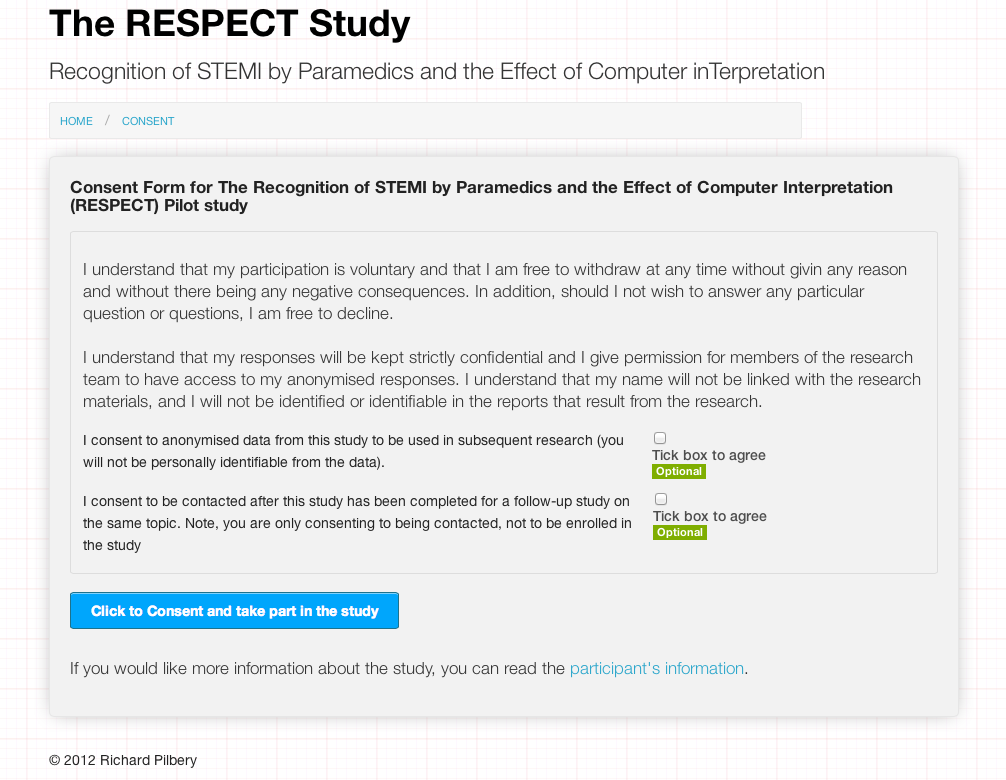
\includegraphics[keepaspectratio,width=1.0000\textwidth,height=0.75\textheight]{consent-screen.png}
\caption{Online consent form for RESPECT pilot study}
\label{consentform}
\end{figure}



\section{Research tool}
\label{researchtool}

Since it was anticipated that participants would be geographically dispersed, an online assessment tool was identified as the most efficient method to collect the data. Existing services were examined, including \href{http://www.surveymonkey.com}{Survey Monkey}\footnote{\href{http://www.surveymonkey.com}{http:/\slash www.surveymonkey.com}} and the forms tool in the \href{http://docs.google.com}{Google Docs}\footnote{\href{http://docs.google.com}{http:/\slash docs.google.com}} suite, but none met the needs of the study. Instead, a custom website was created by the researcher, coded using a \href{http://php.net}{PHP}\footnote{\href{http://php.net}{http:/\slash php.net}} framework, \href{http://cakephp.org}{cakePHP}\footnote{\href{http://cakephp.org}{http:/\slash cakephp.org}}, with a \href{http://www.mysql.com}{MySQL}\footnote{\href{http://www.mysql.com}{http:/\slash www.mysql.com}} database to record and collate the data. To ensure maximum browser and device capability, the Zurb \href{http://foundation.zurb.com}{Foundation}\footnote{\href{http://foundation.zurb.com}{http:/\slash foundation.zurb.com}} responsive front-end framework was used.

In an effort to make the ECGs used in the study as life-size as possible, participants were not permitted to use mobile devices, such as smart phones and tablets, to undertake the study. The study tool calculated the correct size to display the ECGs, based on the participant's computer screen size and resolution. This was achieved by asking participants to resize a virtual bank card displayed on the screen, to a real bank or ID card that they placed on the screen (\autoref{calibrationscreen}). Once this was submitted by the participant, the correct dimensions of the ECG image were calculated.

\begin{figure}[htbp]
\centering
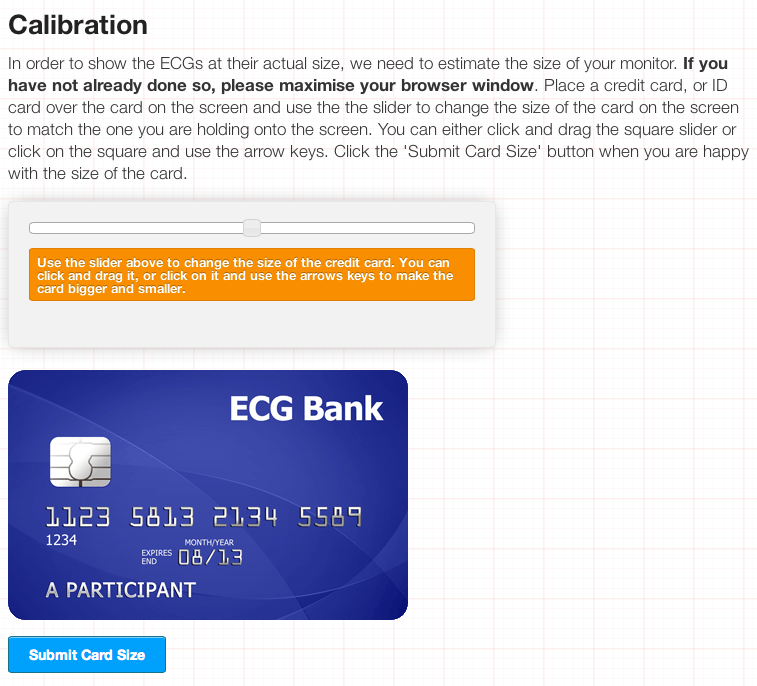
\includegraphics[keepaspectratio,width=1.0000\textwidth,height=0.75\textheight]{calibration.png}
\caption{The RESPECT study calibration screen}
\label{calibrationscreen}
\end{figure}



\subsection{Randomisation}
\label{randomisation}

The study website obtained random numbers from the true random number service \href{http://www.random.org}{RANDOM.ORG}\footnote{\href{http://www.random.org}{http:/\slash www.random.org}}, which generates random numbers from atmospheric noise. These were then utilised by the website to allocate ECGs to participants, to determine ECG and message visibility order, and determine the block randomisation sequence. 

\section{Procedure}
\label{procedure}

The participant flow through the study is shown in \autoref{partsummary}. Paramedics interested in taking part in the pilot study, were invited to visit the study website, read the participant information and enter a contact email address on the sign-up form. Once completed, the website created an entry for the potential participant and sent them an email containing a unique uniform resource locator (URL) web link, as well as links to the participant information sheet and webpage. When the participant clicked the link within the email, they were directed to the consent page (\autoref{consentform}), where informed consent was considered to have been obtained once participants submitted the consent form. Participants were also asked to optionally consent to the use of their anonymised data in subsequent research, and to be contacted about becoming involved in a future, qualitative, study.

\begin{figure}[htbp]
\centering
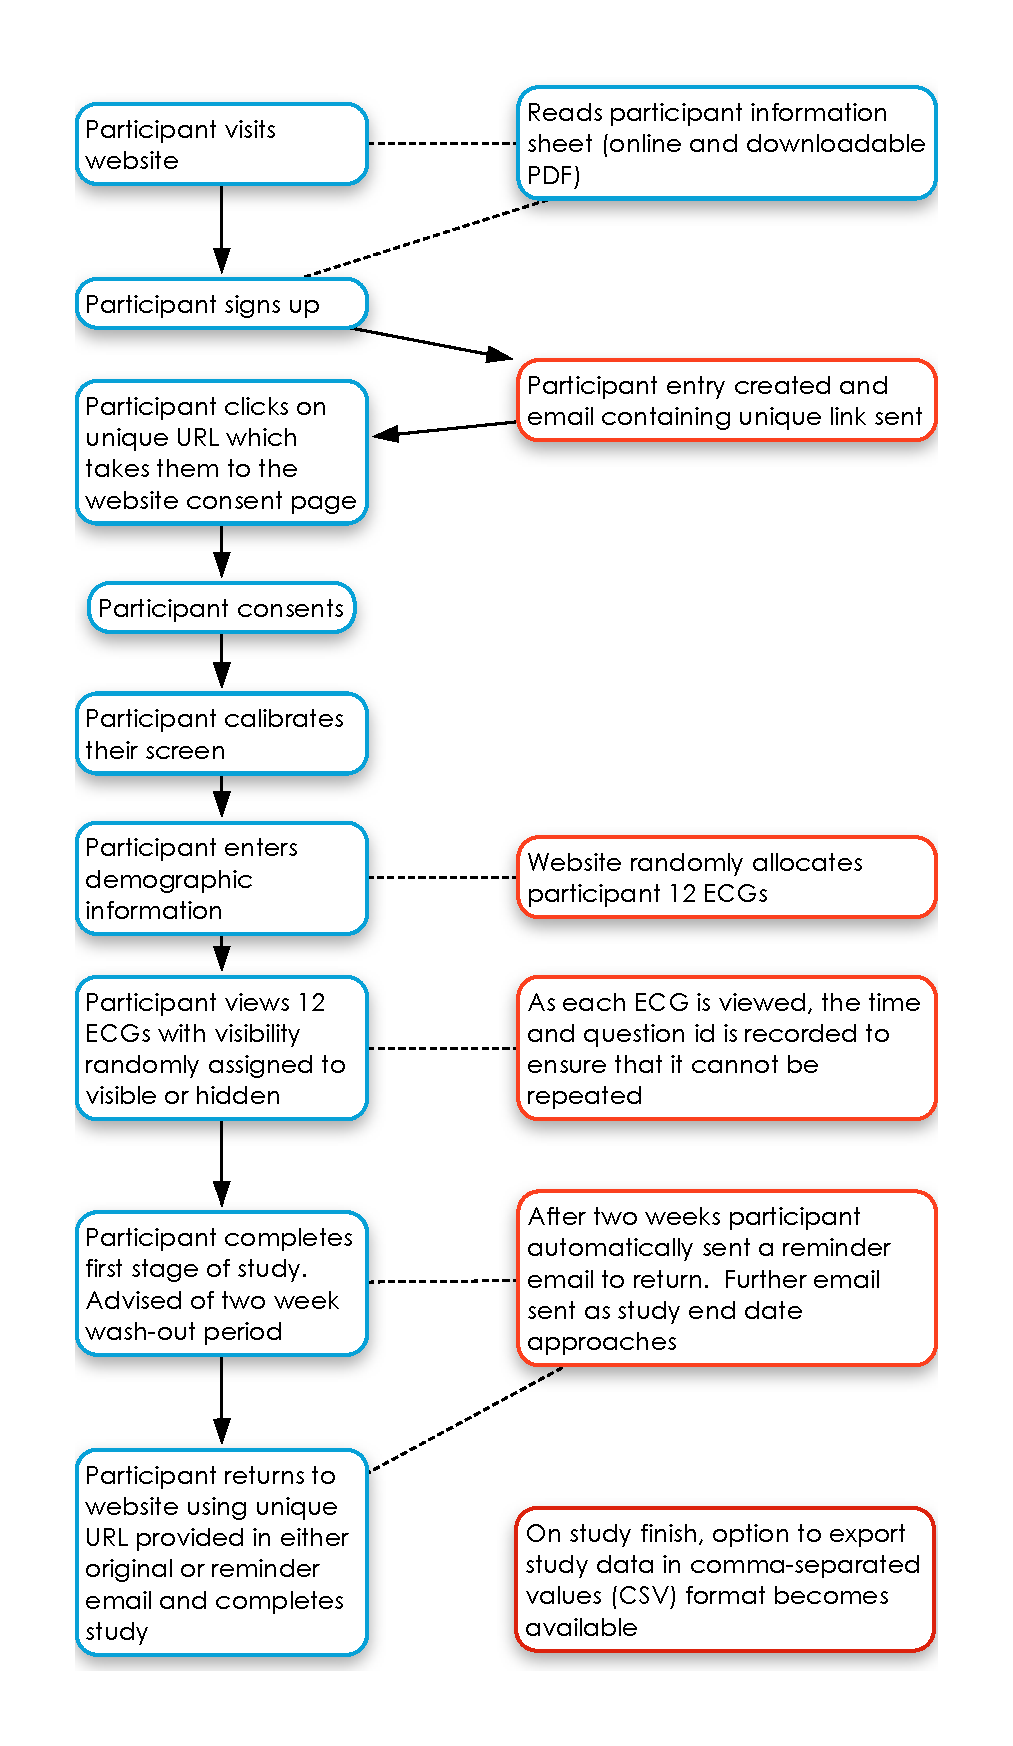
\includegraphics[keepaspectratio,width=\textwidth,height=0.9900\textheight,]{Participant-flow.pdf}
\caption{Flow of participant and website actions during the study}
\label{partsummary}
\end{figure}



After consenting, the participants calibrated their monitor. If the website was accessed using a tablet or mobile device, participants were informed that this could not be used to complete the study, and they were advised to use a desktop or laptop computer. 

The next step was to gather some basic demographic data about the participants, which took the form of four questions:

\begin{enumerate}
\item Which educational route did you take to become a paramedic (traditional\slash vocational, university)

\item How long have you been a paramedic (in years)?

\item How much time have you spent on 12-lead ECG training\slash continuous professional development (CPD) in the past 12 months (in hours)?

\item How many patients have you taken for primary percutaneous coronary intervention or thrombolysed in the past 12 months?

\end{enumerate}

Once completed, participants were randomly allocated 12 ECGs from the study pool of 48. These included three ECGs from each of the following four sub-groups:

\begin{itemize}
\item Patient has a STEMI and computer interpretation states STEMI (true positive)

\item Patient does not have a STEMI and computer interpretation states STEMI (false positive)

\item Patient has a STEMI and computer interpretation states no STEMI (false negative)

\item Patient does not have a STEMI and computer interpretation states no STEMI (true negative).

\end{itemize}

Note that the terms in brackets (e.g. true positive) refer to the computer interpretation in relation to the reference standard.

The ECGs were displayed on a pop-up webpage (\autoref{ecgform}), complete with countdown timer and a form to record the participant responses.

\begin{figure}[htbp]
\centering
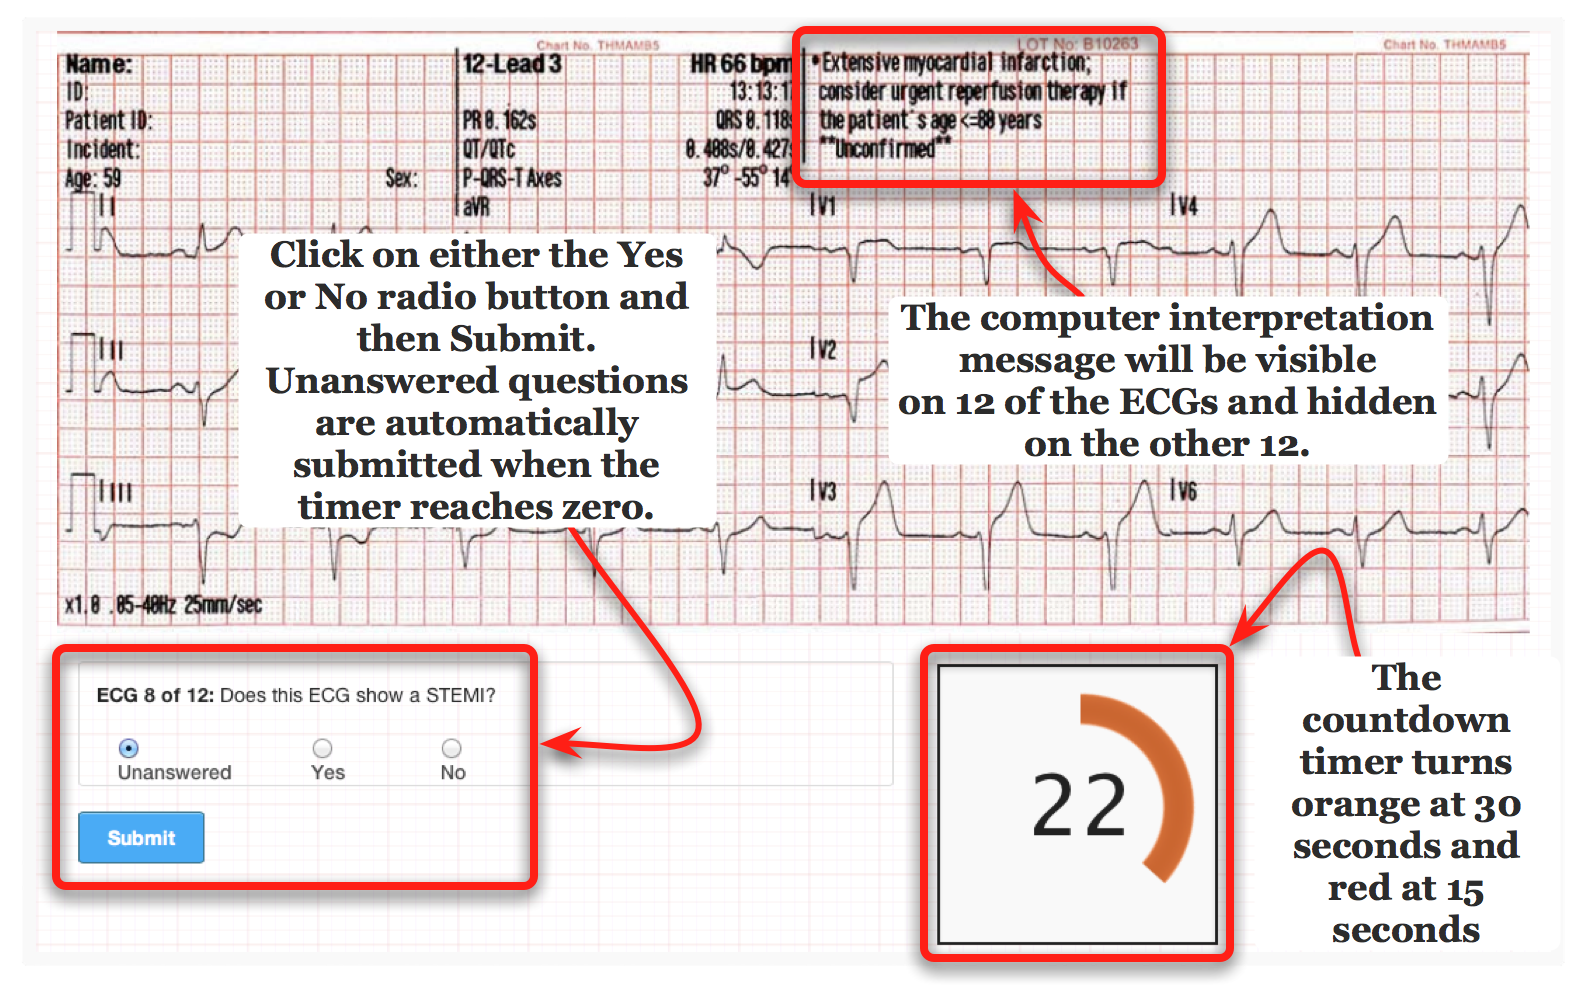
\includegraphics[keepaspectratio,width=1.0000\textwidth,height=0.75\textheight]{ecg-explain.png}
\caption{The RESPECT study ECG webpage}
\label{ecgform}
\end{figure}



Each ECG was viewed by the participant twice, once with and without the message, and the order that these ECGs were shown, was randomised. Participants were informed that the ECGs would be a mixture of STEMI and STEMI-mimic patterns, but not how many of each would be seen. In addition, they were advised that after the wash-out period, they would see the same ECGs again, but with the message visibility reversed. Incentives for completion were randomised in the pilot study, with participants either offered a CPD certificate, entered into a prize draw to win an paramedic textbook, or nothing.

To ensure that all ECGs were viewed in roughly equal numbers, block randomisation of the ECGs was used~\citep{sedgwick_block_2011}. This meant that all 48 ECGs were allocated after every forth participant, assuming that they completed the study. To minimise the chance of subversion bias, allocation was completely automated and the researcher unaware of the randomisation sequence~\citep{torgerson_designing_2008}.

Once the allocation of ECGs was completed, participants were presented with 12, 12-lead ECGs, each having a time limit of 60 seconds to interpret the ECG and submit a response. As soon as an ECG was displayed on the participant's screen, the record for that attempt was updated and no subsequent attempt was allowed, even if the participant failed to answer the question. After 60 seconds, or on submission of the form on the page, the ECG and submission form were removed from the screen and the participant was invited to view the next ECG. 

Once the first 12 ECGs had been reviewed, participants were given a two-week wash-out period and not allowed to progress until this time period had elapsed. Once the wash-out period was over, participants were contacted by email and invited to take part in the second phase (i.e. the crossover). Participants reviewed the same 12 ECGs as before, but in a random order, and with the computer message visibility the opposite of that viewed in the first phase. 

\section{Analysis plan}
\label{analysisplan}

\subsection{Data checking}
\label{datachecking}

Prior to analysing the results, the data was checked to ensure that categorical data (training route and the ECG answers) had allowed values, and numerical variables (CPD hours, service years, number of thrombolysis\slash pPCI patients) were within appropriate ranges. In addition, question start and finish times were reviewed to ensure that finish times occurred after start times. 

\subsection{Missing data}
\label{missingdata}

Due to the crossover nature of the design, each ECG viewed by an individual participant should have a paired response. Where this did not occur, the responses for the specific individual were excluded. This was on the basis that the data were unlikely to be missing at random and the statistical analysis required to account for this is well beyond the capabilities of a non-statistician~\citep{ho_dropouts_2012}. In addition, continuing with the analysis on the assumption that the data was missing at random would have resulted in bias~\citep{baraldi_introduction_2010}.

Responses which timed out (i.e. were not answered within 60 seconds) were coded differently in order to differentiate them from active participants responses. However, for the analysis, these were treated as providing an incorrect answer on the basis that a delayed response reflected the participant's uncertainty regarding the interpretation. 

\subsection{Data description}
\label{datadescription}

Since the data were clustered around participants (who viewed multiple ECGs) and ECGs (which were viewed by multiple participants), a modified Consolidated Standards of Reporting Trials (CONSORT) flow diagram~\citep{campbell_consort_2012} was created to clearly identify participant flow through the study, and provide summary information for the ECGs, including details about the characteristics of the clusters. 

\subsection{Participants}
\label{participants}

As part of the consenting process, participants were asked if they were prepared to allow their anonymised data to be used in future studies, and for permission to contact them for a subsequent, qualitative study. Since the demographic-type data collected from participants was not expected to be normally distributed, it was summarised using median values. 

\subsection{Electrocardiograms}
\label{electrocardiograms}

Two summary tables containing participant responses for each of the ECGs was created to provide overall completion rates for individual ECGs and a descriptive analysis of the responses. These tables are best utilised alongside the summary ECG data in \autoref{appendixa}, which provides the characteristics of the ECGs themselves, including the classification and the actual, and computer, interpretation. 

\subsection{Data analysis}
\label{dataanalysis}

Statistical data analysis was conducted using the \href{http://www.r-project.org}{R}\footnote{\href{http://www.r-project.org}{http:/\slash www.r-project.org}} statistics package and proceeded in an incremental fashion, commencing with the calculation of participant accuracy, sensitivity and specificity values and intra-class correlation coefficients, before fitting generalised linear regression models (GLM) with and without random effects (multilevel) modelling, to take account of the clustering of data around the participants and ECGs~\citep{petrie_medical_2000}. Although it is not possible to analyse the results of these models, due the lack of \emph{a priori} power calculations, it provided an opportunity to test the analysis methods that will be adopted in the main study. The results of the GLM analysis were verified with another statistics package, \href{http://www.bristol.ac.uk/cmm/software/mlwin/}{MLWin}\footnote{\href{http://www.bristol.ac.uk/cmm/software/mlwin/}{http:/\slash www.bristol.ac.uk\slash cmm\slash software\slash mlwin\slash }}, using the procedure described in \autoref{appendixb}.

\subsubsection{Hypotheses}
\label{hypotheses}

The following hypotheses are to be tested in the main study, and so were tested in the pilot study, to ensure that accurate data preparation and analysis could be conducted:

\begin{quote}

Null hypothesis \textbf{1} - Computer interpretation messages have no effect on paramedics' correct diagnosis of STEMI from a 12-lead ECG 

Alternative hypothesis \textbf{1} - Computer interpretation messages have an effect on paramedics' correct diagnosis of STEMI from a 12-lead ECG.
\end{quote}

The first hypothesis includes all computer interpretation messages, irrespective of classification (true positive, false positive etc). However, the subsequent hypotheses (2 and 3), aim to examine two subsets of the data: accurate (true positive and true negative) and inaccurate (false positive and false negative) computer interpretations: 

\begin{quote}

Null hypothesis \textbf{2} - \emph{Accurate} computer interpretation messages have no effect on paramedics' correct diagnosis of STEMI from a 12-lead ECG 

Alternative hypothesis \textbf{2} - \emph{Accurate} computer interpretation messages have an effect on paramedics' correct diagnosis of STEMI from a 12-lead ECG

Null hypothesis \textbf{3} - \emph{Inaccurate} computer interpretation messages have no effect on paramedics' correct diagnosis of STEMI from a 12-lead ECG 

Alternative hypothesis \textbf{3} - \emph{Inaccurate} computer interpretation messages have an effect on paramedics' correct diagnosis of STEMI from a 12-lead ECG.
\end{quote}

\subsubsection{Generalised linear modelling}
\label{generalisedlinearmodelling}

Regression models that require a transformation (via a link function) of the outcome are known as generalised linear models (GLM). For the binary outcome of a correct (or incorrect) diagnosis, logistic regression was used. Logistic regression is so called because the link function is the logit (or log odds)~\citep{kirkwood_essential_2003}. Thus the first model to be tested (which ignores the clustering of ECGs and participants) takes the form:

\[  logit(\pi) = log\left(\frac{\pi}{(1-\pi)}\right)=\beta_0+\beta_1MESSAGE \] 

where $ \pi $ is the probability of a correct answer when the message is visible, $ \beta $s are the regression coefficients and MESSAGE denotes whether the message is visible (1) or hidden (0)~\citep{campbell_medical_2007}. All data and sub-groups, consisting of accurate computer interpretation only and inaccurate computer interpretation only, were modelled. The Odds ratio, regression coefficient standard error and 95\% confidence interval, z statistic and p-values were calculated and summarised. 

\subsubsection{Generalised linear modelling with random effects}
\label{generalisedlinearmodellingwithrandomeffects}

Regression modelling assumes that the outcome and parameters are independent and identically distributed~\citep{goldstein_multilevel_2002}. However, that is not the case in this study, as each participant response is clustered around the participant and the ECG. Ignoring clustering generally leads to underestimation of regression coefficient standard errors, which in turn leads to overly narrow confidence intervals, and p-values which are too small. Ultimately, coefficients could erroneously be assumed to be significant effects, when in fact the results occurred by chance~\citep{clements_using_2007}.

Clustering can be accounted for by adding random effects to the model. This is achieved by the inclusion of a parameter which varies randomly between clusters, and is assumed to be normally distributed with a mean zero, and a variance equal to the intra-parameter variance. Including random effects in this way, allows observations within the same cluster to be assumed to be independent. Models using random effects are often called multi-level models, since the observations (a participant's individual response to a single ECG) is nested within clusters of the participant and ECG.

The participants and the ECGs are nested within a hierarchy, with each participant response belonging to a participant and an ECG. This is known as a cross-classified structure~\citep{leckie_cross-classified_2013} and can be expressed, using classification notation~\citep{browne_multiple_2001}, as:

$   y_i \thicksim Binomial(1,\pi_i)  $

$ logit(\pi_i) = \beta_0+\beta_1MESSAGE_i+u^{(3)}_{ecg(i)}+u^{(2)}_{participant(i)} $

$  u^{(3)}_{ecg(i)} \thicksim N\left(0,\sigma^2_{u(3)}\right)  $

$   u^{(2)}_{participant(i)} \thicksim N\left(0,\sigma^2_{u(2)}\right)  $

where $  u^{(3)}_{ecg(i)} $ is the random effect for ecg(i), and is assumed to be normally distributed with a mean of zero and variance, $ \sigma^2_{u(3)} $. Likewise, $  u^{(3)}_{participant(i)} $ is the random effect for participant(i), and is assumed to be normally distributed with a mean of zero and variance, $ \sigma^2_{u(2)} $.

\subsubsection{Intra-class correlation coefficients}
\label{intra-classcorrelationcoefficients}

The intra-class correlation coefficient (ICC) is a measure of the degree of similarity in ECG interpretation attempts within a cluster~\citep{eldridge_intra-cluster_2009}, and is used to calculate the design effect, by which sample size estimates are multiplied, in order to account for clustering~\citep{yelland_adjusted_2011}.

Three ICCs were calculated from the random effects models. The first, examined the correlation between two randomly selected responses from the same participant:
\[ \frac{\sigma^2_{participant}}{\left(\sigma^2_{ecg}+\sigma^2_{participant}+\frac{\pi^2}{3}\right)} \]

The second ICC, measured the correlation between two randomly selected responses from the same ECG:
\[ \frac{\sigma^2_{ecg}}{\left(\sigma^2_{ecg}+\sigma^2_{participant}+\frac{\pi^2}{3}\right)} \]

Finally, the correlation between two randomly selected responses from the same participant, and same ECG (sometimes called the interaction ICC) was calculated:
\[ \frac{\sigma^2_{ecg}+\sigma^2_{participant}}{\left(\sigma^2_{ecg}+\sigma^2_{participant}+\frac{\pi^2}{3}\right)} \]

In all cases, $  \sigma^2_{participant} $ is the variance between participants, $  \sigma^2_{ecg} $ the variance between ECGs and $  \frac{\pi^2}{3} $ is the residual variance for a logit model. 

\subsubsection{Incentives}
\label{incentives}

Participants who consented to take part in the study were randomly assigned one of three incentive options (no incentive, a downloadable continuing professional development certificate and a prize draw for a paramedic textbook). A participant was eligible for the incentive IF they completed both parts of the study. To determine the potential impact of offering incentives on retention, the following hypothesis was proposed:

\begin{quote}

Null hypothesis \textbf{4} - The proportion of study completion does not differ between the incentive options

Alternative hypothesis \textbf{4} - The proportion of study completion is different between the incentive options.
\end{quote}

This was tested using a chi-squared test for independence. 

\section{Limitations and potential problems}
\label{limitationsandpotentialproblems}

Since this study is a pilot, the results, will require confirmation in a subsequent study~\citep{torgerson_designing_2008}. No clinically important results were determined prior to the study commencement, which means that an appropriate sample size calculation to improve statistical rigour, was not calculated.

Recruiting participants was anticipated to be a significant problem~\citep{watson_increasing_2006}. Although there was an incentive, it could not be advertised, since 1 in 3 participants were not going to receive one. Given that there was no budget for marketing, social networking tools were utilised, including \href{http://twitter.com}{Twitter}\footnote{\href{http://twitter.com}{http:/\slash twitter.com}}, the \href{http://www.ukambulanceforum.com}{UK Ambulance Forum}\footnote{\href{http://www.ukambulanceforum.com}{http:/\slash www.ukambulanceforum.com}} and personal contacts throughout the UK. In addition, support was obtained from the College of Paramedics who advertised the study on the \href{https://www.collegeofparamedics.co.uk/home/}{College website}\footnote{\href{https://www.collegeofparamedics.co.uk/home/}{https:/\slash www.collegeofparamedics.co.uk\slash home\slash }}.

There was a risk that the web-based assessment tool could prove difficult to use and\slash or suffer from technical glitches, making data collection problematic. However, the tool was extensively tested prior to the start of the pilot to ensure it captured data reliably. Furthermore, limited usability testing on paramedics who were not taking part in the pilot study was undertaken to ensure that the instructions were clear and the assessment tool straightforward to use. These issues are precisely why conducting a pilot study is a good idea, and should ensure that the tool is robust enough for use in the main study.

With a web-based assessment tool, there was a risk that the participant might have utilised a textbook or sought advice from others. In order to minimise this, a unique universal resource locator (URL) was included in the emails sent to each participant, preventing unauthorised access to the study website. In addition, each ECG, once viewed by the participant, could not be answered again, and a time limit was imposed for each question, after which the website automatically removed the ECG and the response form from view.

The study's crossover design required participants to return to the website, to repeat the assessment, two weeks after completing the first stage. This did present an issue, since if participants did not return, then there would be no paired data to analyse. In an effort to minimise this, automatically generated emails were sent to participants, reminding them to return to the study, and the aforementioned social networks were utilised in an ongoing effort not just to recruit new participants, but also to encourage existing participants to return after the wash-out period.

\section{Methods of dissemination}
\label{methodsofdissemination}

The results of the study are presented and discussed in detail in \autoref{results}. Since consent was obtained from participants to use an anonymised version of the dataset in subsequent research, the data will be made publicly available online, via the study website, to promote data sharing~\citep{ross_importance_2012}. However, in an attempt to reduce the likelihood of post-hoc data analysis (data-dredging)~\citep{lord_multiple_2004}, researchers who wish to access the study data will be required to submit a study protocol to the RESPECT chief investigator. In addition, to enable the research to be reproducible, a full summary of the statistical analysis will be presented using the R statistics package \href{http://yihui.name/knitr/}{knitr}\footnote{\href{http://yihui.name/knitr/}{http:/\slash yihui.name\slash knitr\slash }}, which enables a researcher to present the R scripts which conduct the analysis, and the results of that analysis, together (an example can be found in \autoref{appendixi}). More conventional methods of dissemination will also be utilised, including publishing findings in a peer-reviewed journal, such as the \emph{Emergency Medicine Journal}, presenting at conferences, and the publication of plain English summaries in the College of Paramedics newsletter and free ambulance magazines. 

\section{Timetable}
\label{timetable}

\autoref{gantt} shows the planned timeline for the RESPECT pilot study, which commenced in September 2012 and finished with the dissertation write up and submission towards the end of September, 2013. Regular meetings were scheduled with the dissertation supervisor. In addition, a statistician was periodically consulted during the design and analysis stages.

 \begin{figure}[htbp] 

 \centering 

 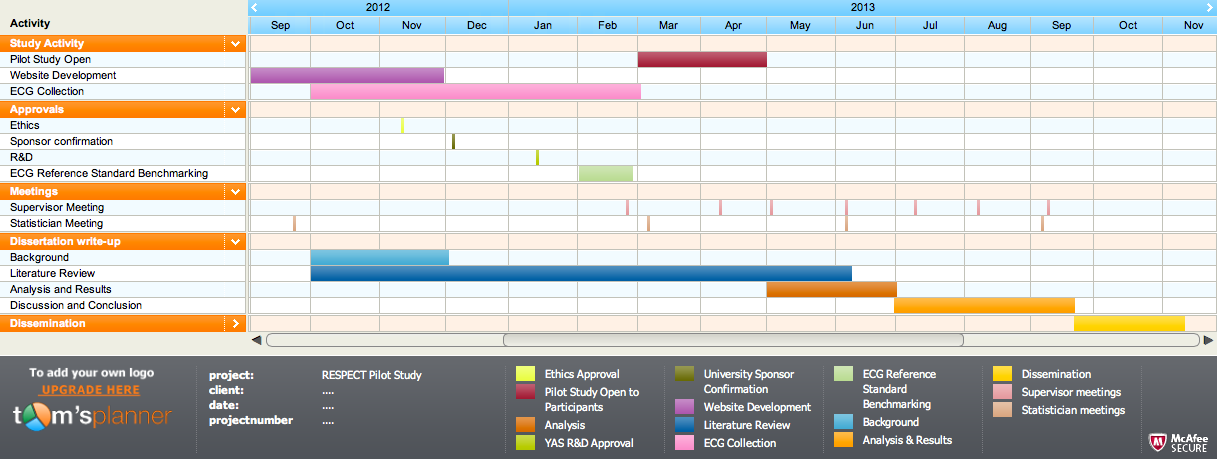
\includegraphics[keepaspectratio,width=1.50\textwidth,height=1.00\textheight, angle=90]{Gantt.png}  

 \caption{Gantt chart for RESPECT pilot study}  

 \label{gantt}  

 \end{figure}  
